\chapter{Spectroscopic Sky Surveys}
\label{data_chapter}

% TODO chapter summary

Select suitable dataset of astronomical spectra for experiments.

To understand this work we need first to introduce the spectral
data because we are interested in classifying them.

\section{Astronomical Spectroscopy}

Spectroscopy started when Issac Newton carried out the experiment of light decomposition throgh a prism in 1666.
Next, Thomas Young has shown that light behaves like a wave.
The wave nature of light allowed Joseph von Fraunhofer to invet the diffraction grating.
Diffraction gratings are one of the essential parts of modern spectroscopes
because they allow greater dispersion than prisms.
Fraunhofer was also one of the first to observe dark lines in the solar spectrum.
David Brewster postulated that the dark lines correspond to absoption from gas in the way of light travelling towards us.
Robert Wilhelm Bunsen and Gustav Kichhoff showed that each chemical element has its own set of spectral lines.
Therefore, spectrocopy can be used for chemical analysis of matter.
Kichhoff established the three famous laws describing the three types of spectra:
continuous, emission and absorption.
Joseph von Fraunhofer was the first to observe spectra of stars by using spectroscope in combination with telescope.
Christian Doppler discoverd the Doppler effect that allowed to measure the motion of celestial objects using Doppler shift in its spectrum.
Then, at the beginning of the twentieth century,
the invention quantum mechanics help us to understand the origin of spectral lines.
Max Planck derived the spectral distributon of a black body.
Ludwig Boltzmann, Joseph Stefan, Wilhelm Wien, Niels Bohr etc.
Nowadays, new technologies have advanced spectroscopic observations
(CCD detectors, optical fibers and computing power).~\cite{cochard2018}

\begin{figure}
	% source https://solarsystem.nasa.gov/resources/390/the-solar-spectrum/
	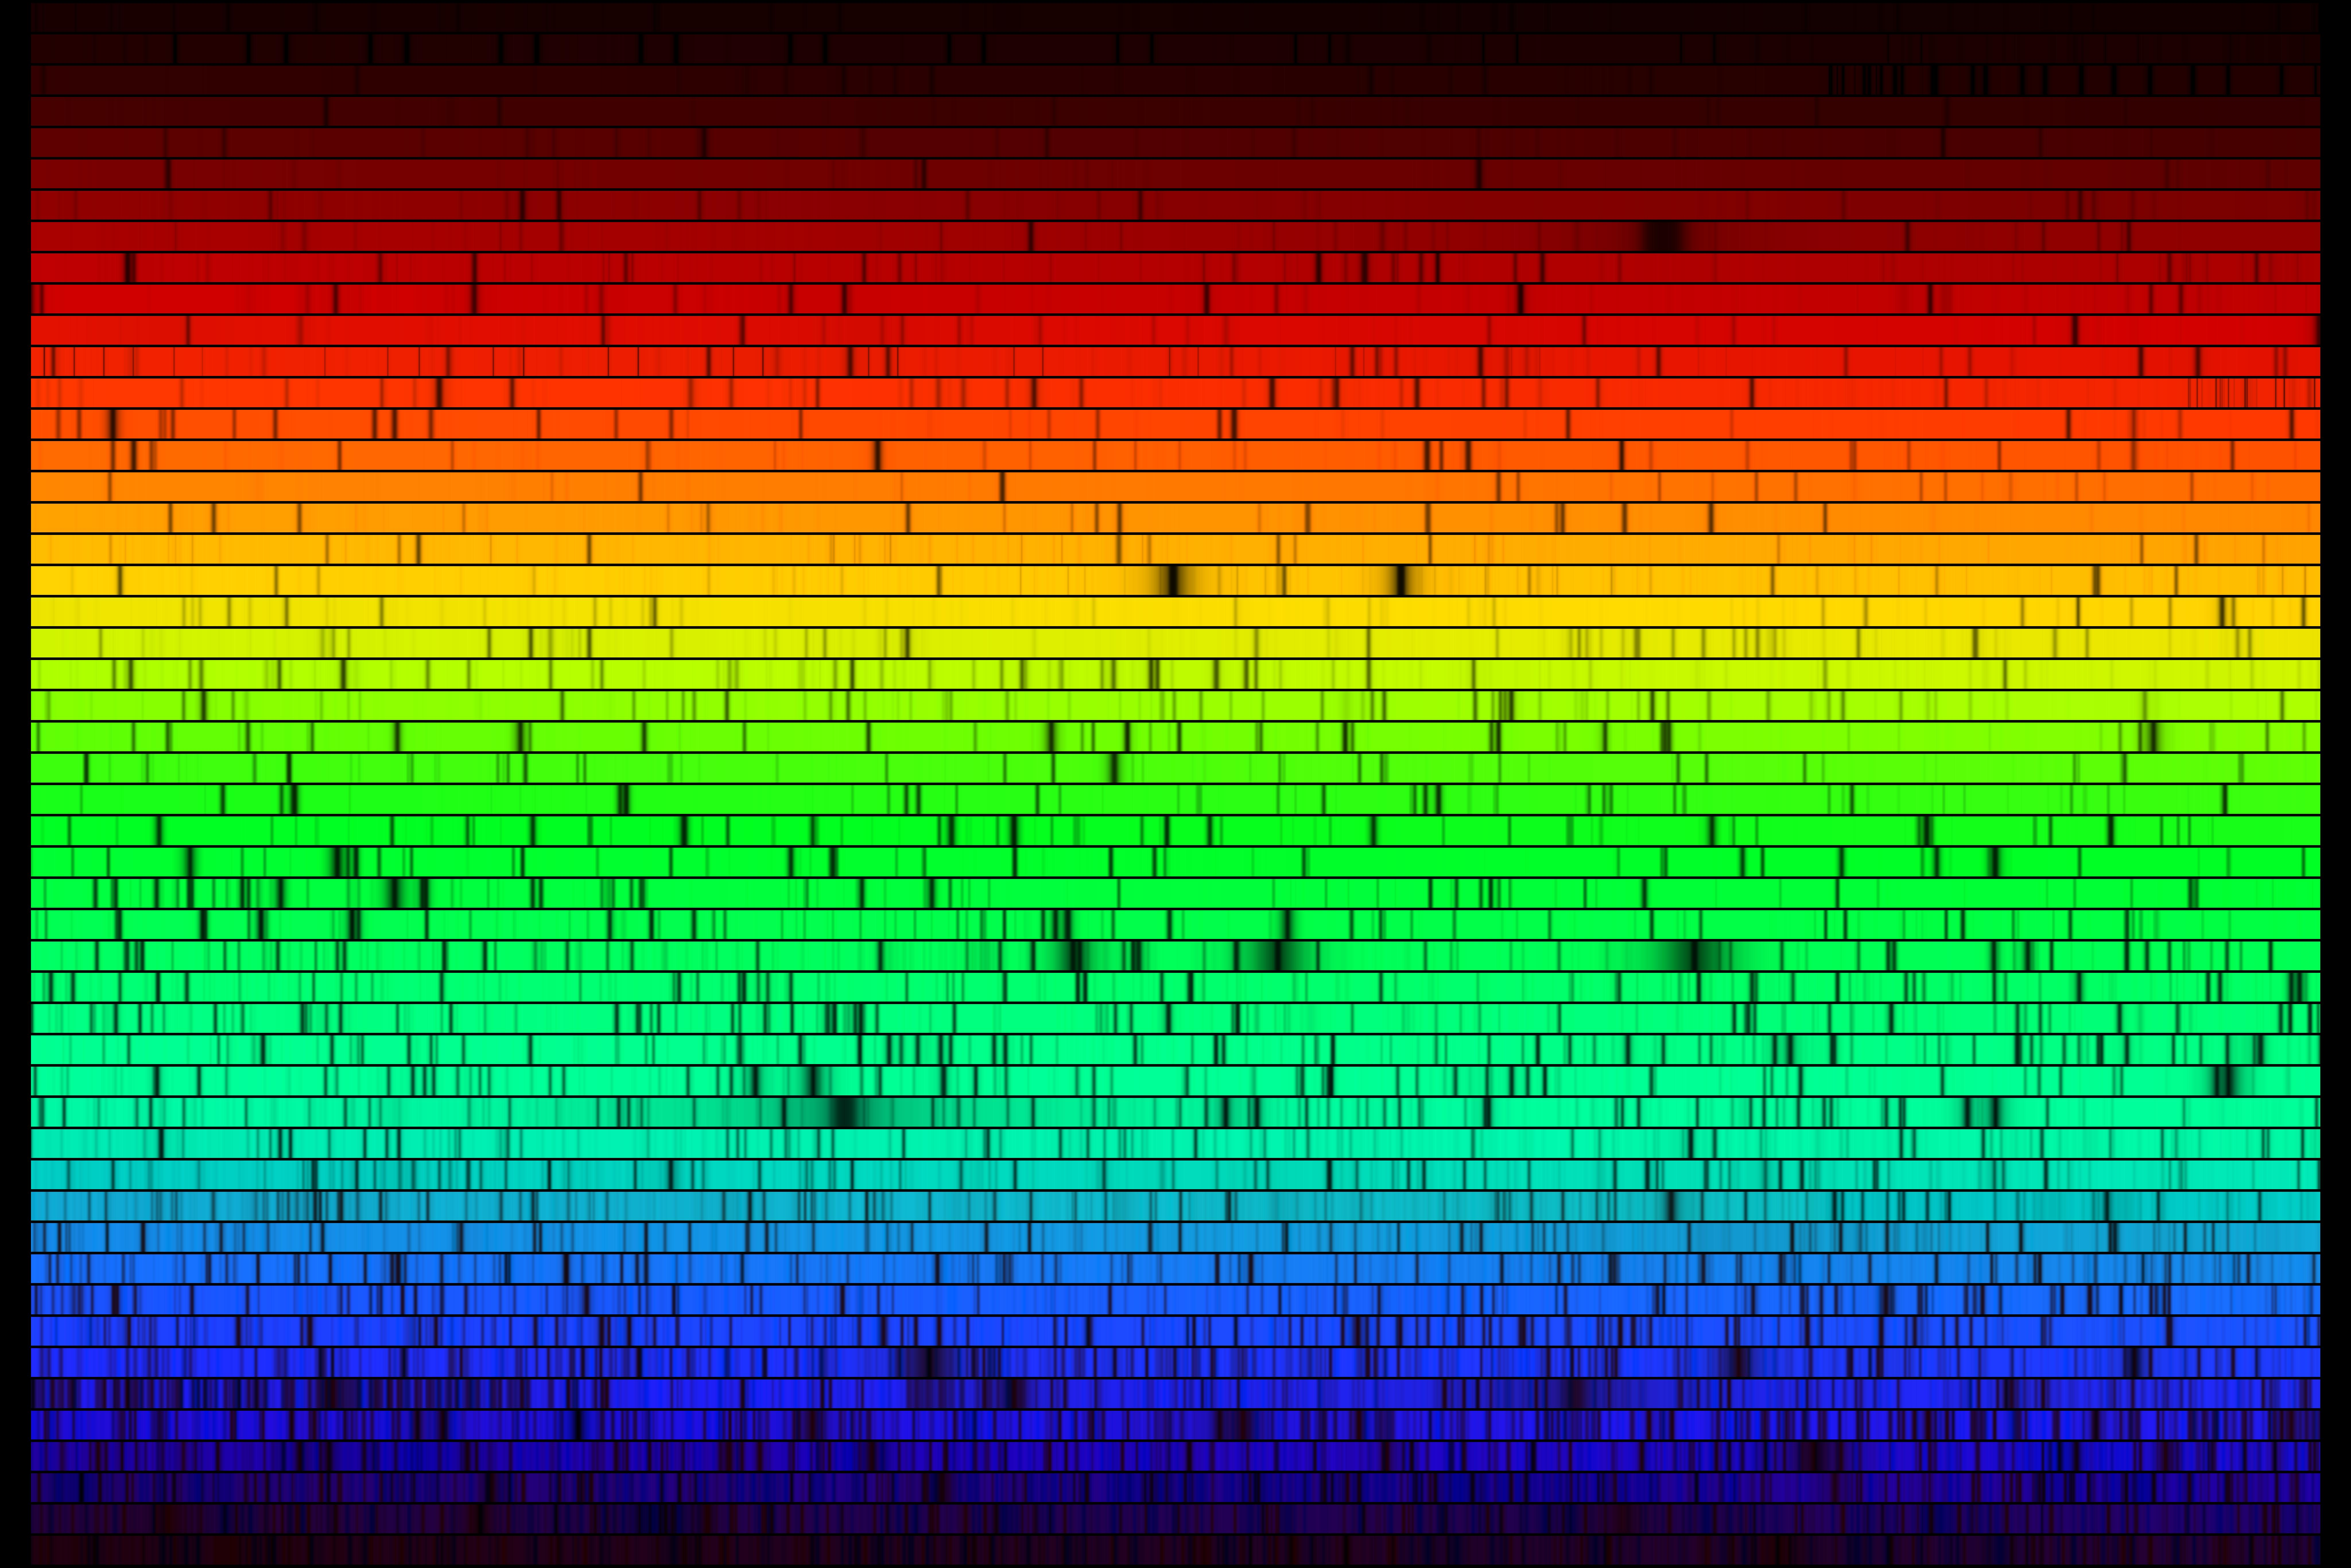
\includegraphics[width=\textwidth]{img/solarspectrum.jpg}
	\caption{The Solar Spectrum (Image by \href{https://solarsystem.nasa.gov/resources/390/the-solar-spectrum/}{NASA})}
	\label{solar_spectrum}
\end{figure}

Almost all we know about the universe outside our solar solar is based on the analysis of electromagnetic radiation.
We have derived information by observing flux, time variations, etc.~\cite{appenzeller2012}

Light is an electromagnetic wave that can be decomposed (by a prism or a diffraction grating) as a function of its wavelength.
The decomposition is called spectrum.
Electromagnetic wave propagetes in the speed of light \(c\).
The electromagnetic wave transfers energy
(the higher the frequency the more energy it carries).~\cite{cochard2018}

Secondly, light is a beam of photons: particles of light.
Photons has no mass but transport energy and have momentum.
Every photon has an associated frequency \(\nu\) of the corresponding electromagnetic wave giving it a energy \(E = h \nu\).

Matter is made of atoms.
An atom has a specific number of electrons which are place in particular orbits of the atom.
Electrons in an orbit have a specic energy level.
We know from quantum mechanics that an electron can change energy level by an exchange of energy in form of a photon.
The energy transfer is not continuous.
The energy has to precisily correspond to the difference in the energy levels.
Therefore the change produces a light with an energy \(E\) in the wavelegth \(\lambda\):

\begin{equation}
	\lambda = c \frac{h}{E}.
\end{equation}

Therefore, the specific set of energy levels of a atom detemines photons either abosrbed or emitted by it.
This is a direct consequence for spectroscopy.~\cite{cochard2018}

Black body radiation.
Light is produced by either heating up matter or by exciting atoms.
Heating transforms into an emission of light at all wavelengths with an energy distribution (a function of wavelength) which only depends on the temperature.
Planck's law:

% https://en.wikipedia.org/wiki/Planck%27s_law
\begin{equation}
	B_{\lambda}(\lambda, T) = \frac{2 h c^2}{\lambda^5} \frac{1}{e^{\frac{hc}{\lambda k_{\mathrm{B}}T}} - 1}
\end{equation}

where \(k_{\mathrm{B}}\) is the Boltzmann constant.
This phenomenon does not depend on the composition of the body.
The Wien's displacement law gives the wavelength of maximum intensity \(\lambda_{\max}\):

\begin{equation}
	\lambda_{\max} = \frac{b}{T}
\end{equation}

where \(b\) is the Wien's displacement constant.
Similarly, we can derive the temperature \(T\) with known wavelength of maximum intesity \(\lambda_{\max}\):

\begin{equation}
	T = \frac{b}{\lambda_{\max}}.
\end{equation}

where \(b\) is the Wien's displacement constant.~\cite{cochard2018}

Secondly, light can be emitted by exciting atoms.

Photons carry information about the observed object to a pixel of a \textit{charge-coupled device} (CCD) camera.
Electomagnetic radiation exhibits both wave and particle nature throughout the entire spectra
(\(\gamma\) rays, X-rays, ultraviolet, visible light, infrared radiation, microwaves, radio waves).
CCD cameras require the particle nature of light (electromagnetic radiation).~\cite{trypsteen2017}

\begin{table}
	\begin{center}
		\begin{tabular}{|l|r|}
			\hline
			Radiation type & Wavelength (m) \\ \hline \hline
			\(\gamma\) ray & \(10^{-12}\) \\ \hline
			X-ray & \(10^{-10}\) \\ \hline
			Ultraviolet & \(10^{-8}\) \\ \hline
			Visible & \(0.5 \times 10^{-6}\) \\ \hline
			Infrared & \(10^{-5}\) \\ \hline
			Microwave & \(10^{-2}\) \\ \hline
			Radio & \(10^{3}\) \\ \hline
		\end{tabular}
	\end{center}
	\caption{Electromagnetic spectrum}
\end{table}

A photon caries a specific energy that match certain frequency.
Higher frequency means higher energy.
All photons always move in the speed of light.
For each wavelength the corresponding photon energy \(E\) is given by the Planck--Einstein relation:

\begin{equation}
	E = h \nu \label{planck_einstein_equation}
\end{equation}

where \(h\) is the Planck constant and \(\nu\) is frequency of the photon.
The frequency \(\nu\) is related to the wavelength \(\lambda\):

\begin{equation}
	\nu = \frac{c}{\lambda} \label{frequency_wavelength_equation}
\end{equation}

where \(c\) is the speed of light.
Combining equations~\ref{planck_einstein_equation} and \ref{frequency_wavelength_equation} gives:

\begin{equation}
	E = h \frac{c}{\lambda}.
\end{equation}

Therefore, the energy of a photon is proportional to its frequency \(\nu\)
and inversly proportional to the wavelength \(\lambda\).~\cite{trypsteen2017}

The blackbody is a physical model for stellar radiation.
Objects hotter than its environment emit electromagnetic radiation.
Objects also reflect radiation.
But stars rather absorb all incomming radiation.
Therefore, we consider the Sun as a blackbody.
A perfert blackbody absorbs all incomming radiation.
Therefore, all its radiation is determined only by its temperature.~\cite{trypsteen2017}

The undisturbed profile of a continuum level \(I_C(\lambda)\) represents roughly the temperature dependence blackbody radiation characteristics \(B_T(\lambda)\).

With the Wien's displacement law we can estimate the absolute temperature \(T\) of a star.

Bolometric energy flow \(F_{\mathrm{bol}}\):

\begin{equation}
	F_{\mathrm{bol}} = \int_0^{\infty} I(\lambda) \mathrm{d} \lambda
\end{equation}

and Stefan--Bolzmann law:

\begin{equation}
	F_{\mathrm{bol}} = \sigma T^4
\end{equation}

where \(\sigma\) is the Stefan--Bolzmann constant.~\cite{trypsteen2017}

Telescopes are giant eyes that can collect much more light that human's eye.
Spectrographs can disperse the light collected by a telescope into spectra
which reveal objects composition, speed, temperature and more.~\cite{bennett2005}

The visible light is only a tiny part of the complete spectrum of electromagnetic radiation.
The complete spectrum of electromagnetic radiation is usually called the electromagnetic spectrum.
Electromagnetic radiation carries information about stars and planets made of matter across the universe.
The energy carried by light interacts with matter in following ways:

\begin{itemize}
	\item \textit{emission} (an electric current flowing through the bulb heats it to a point at
		which its matter emits visible light);
	\item \textit{absorption} (hand placed near a lit light bulb absorbs some of the light).
\end{itemize}

Spectra come in three basic types, and real astronomical spectra are usually a combination of these types:

\begin{itemize}
	\item the spectrum of a conventional light bulb is a continuous rainbow (called \textit{thermal radiation spectrum});
	\item if a cloud of gas lies between a detector and a bulb,
		the cloud can absorb specific wavelength making what an absorption line spectrum;
	\item the cloud might emit light itself; therefore, this spectrum is called an emission-line spectrum.
\end{itemize}

The fact that each atom, ion or molecule possesses a unique set of energy levels
causes emission and absorption lines at specific wavelengths in spectra.
Spectral lines correspond to the wavelengths of light absorbed by chemicals on the surface of the star.
Therefore, positions of emission and absorption lines can tell us objects composition.
We display spectra as bands of light that is a projection of light that passes through a prism on a wall
(see Fig.~\ref{solar_spectrum}):
called \textit{two dimensional} spectra.~\cite{cochard2018}
A more reasonable way is to display spectra as graphs of intensities of the light as the vertical axis and wavelengths as the horizontal axis:
called a \textit{one-dimensional spectral profile}.~\cite{cochard2018}
This representation of a astronomical spectrum can be seen as a one-dimensional image.
Therefore, convolutional neural networks seem to be a great tool to analyse them.~\cite{bennett2005}

% TODO add acronym SNR
Signal-to-noise ratio (SNR) is a parameter of our instrument.
We can tust our measurment when signal is high in compared to nise.~\cite{cochard2018}

\section{Quasi-Stellar Objects}

Quasi-stellar (star-like) objects (also known as \textit{quasars} and abbreviated \textit{QSO}) are the most luminious \textit{active galactic nuclei} (AGNs).~\cite{beckmann2013}

The physical model is a supermassive black hole surrounded by a gaseous accretion disk.
A QSO generates energy by stress and friction in the disk outside ot the black hole because no light can escape the \textit{event horizont}.
The energy is in form of electromagnetic radiation and is the strongest in the ultraviolet band.
Moreover, QSOs exhibit big cosmological redshift.

QSOs were common in the early universe probably because galaxies have run out of matter: they stop to be so lumionious.
Therefore, QSOs help us to study the early universe.

There are different types of QSOs: radio-loud, radio-quiet, broad absorption-line, type II, red, optically violent variable, weak emission-line.

\begin{itemize}
	\item Physical definition of QSOs.
	\item Definition of QSOs according SDSS DR14Q.
	\item Why QSOs are interesting? Something as the expanding Universe.
	\item Why QSOs are suitable for experimenting with DA?
		QSOs have big redshift and CNNs are shift invariant.
		Searching for QSOs in different archives.
\end{itemize}

\begin{figure}
	% TODO align
	\begin{center}
		\subfloat[Best image of bright quasar 3C 273][
			Best image of the bright quasar 3C 273
			(Image by \href{https://www.spacetelescope.org/images/potw1346a/}{ESA/Hubble} is licensed under CC BY 4.0)
			]{
			% TODO give credit https://www.spacetelescope.org/images/potw1346a/
			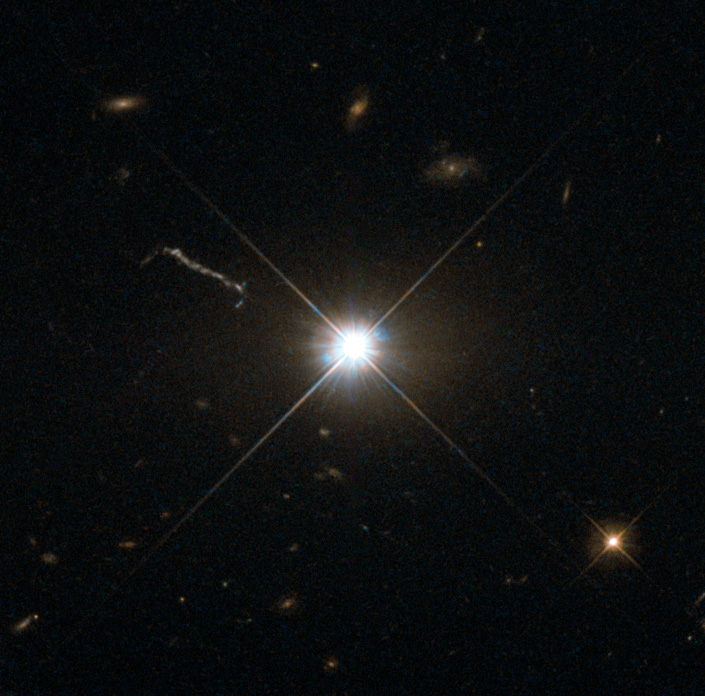
\includegraphics[height=0.45\textwidth]{img/potw1346a.jpg}
			}
		\subfloat[Jet]{
			% TODO give credit https://chandra.harvard.edu/photo/2000/0131/index.html
			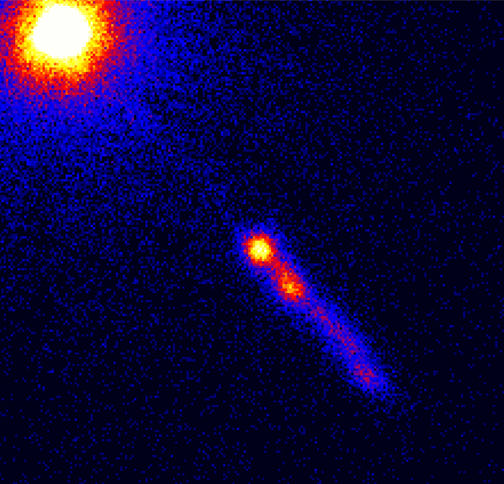
\includegraphics[height=0.45\textwidth]{img/0131_xray.jpg}
			}
	\end{center}
	\caption{
		The first ever discover quasar 3C 273.
		}
	\label{3c_273}
\end{figure}

% TODO include 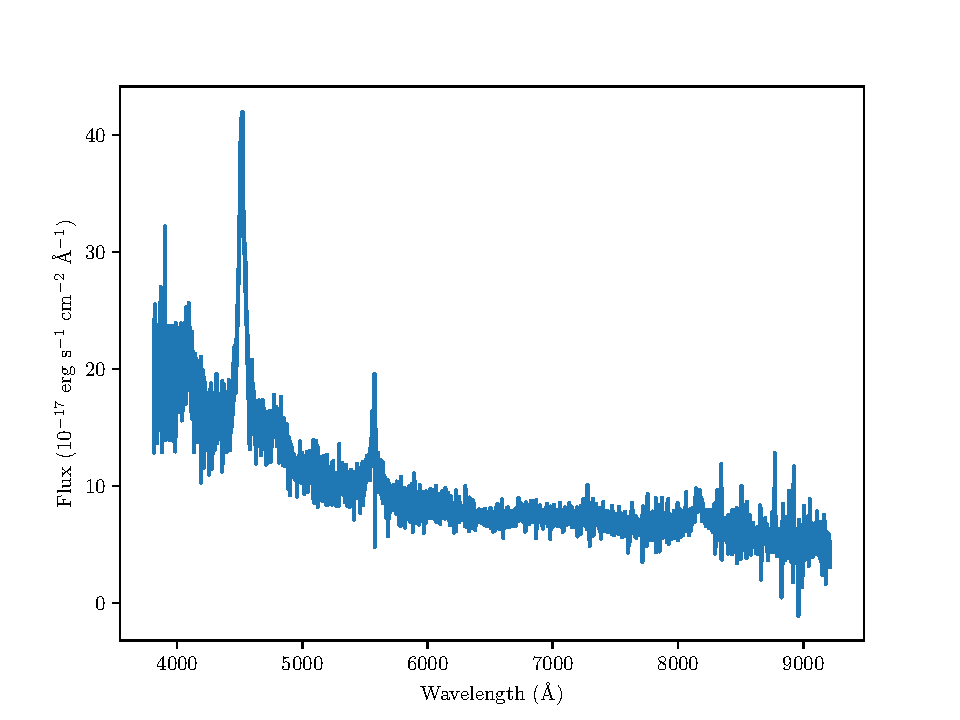
\includegraphics[width=\textwidth]{img/spec_3c_273.pdf}

\section{Large Spectroscopic Surveys}

Give list of large spectral archives focused on observation of QSOs.
Main archives are SDSS and LAMOST.
Gaia doesn't have spectra available yet.
Marginal archives are GALEX (ultraviolet), CALIFA or ESO MUSE.
Spectroscopic surveys mentioned by SDSS DR14Q:

\begin{itemize}
	\item Bright Quasar Survey;
	\item Large Bright Quasar Survey (LBQS); and
	\item 2dF Quasar Redshift Survey.
\end{itemize}

Choose LAMOST and SDSS and tell why we have choosen them.

LAMOST is a stellar and extra-galactic spectroscopic survey.

SDSS is a spectroscopic and optical survey.

CALIFA is a spectroscopic survey of galaxies.

\subsection{Sloan Digital Sky Survey}

Describe SDSS, its spectra and catalog of QSOs.

% TODO clarify what is photometry and astrometry?
The SDSS is designed to provide both a photometrically and astrometrically clalibrated imaging survey
and a spectroscopic survey of galaxies and quasars.~\cite{york2000}

The SDSS survey uses a 2.5~m telescope located at the Apache Point Observatory, New Mexico.
The telescope has 3\(^{\circ}\) fild of view due to the mirror.
The original spectrograph of the telescope was able to obtain 640 spectra
with a wavelength coverage 380--920~nm simultaneously
with spectral resolution \(R \sim 1800\).~\cite{gunn1998, york2000}

In 2009, the original spectrograph was upgraded for Baryon Oscillation Spectroscopic Survey (BOSS).
The upgraded BOSS spectrograph covers a wavelength range 356--1040~nm
with resolving power \(R \sim 2000\)
and is capable to 1000 spectra at once.~\cite{smee2013}

% TODO SDSS has absolute flux calibration while LAMOST does not

\begin{figure}
	% source https://solarsystem.nasa.gov/resources/390/the-solar-spectrum/
	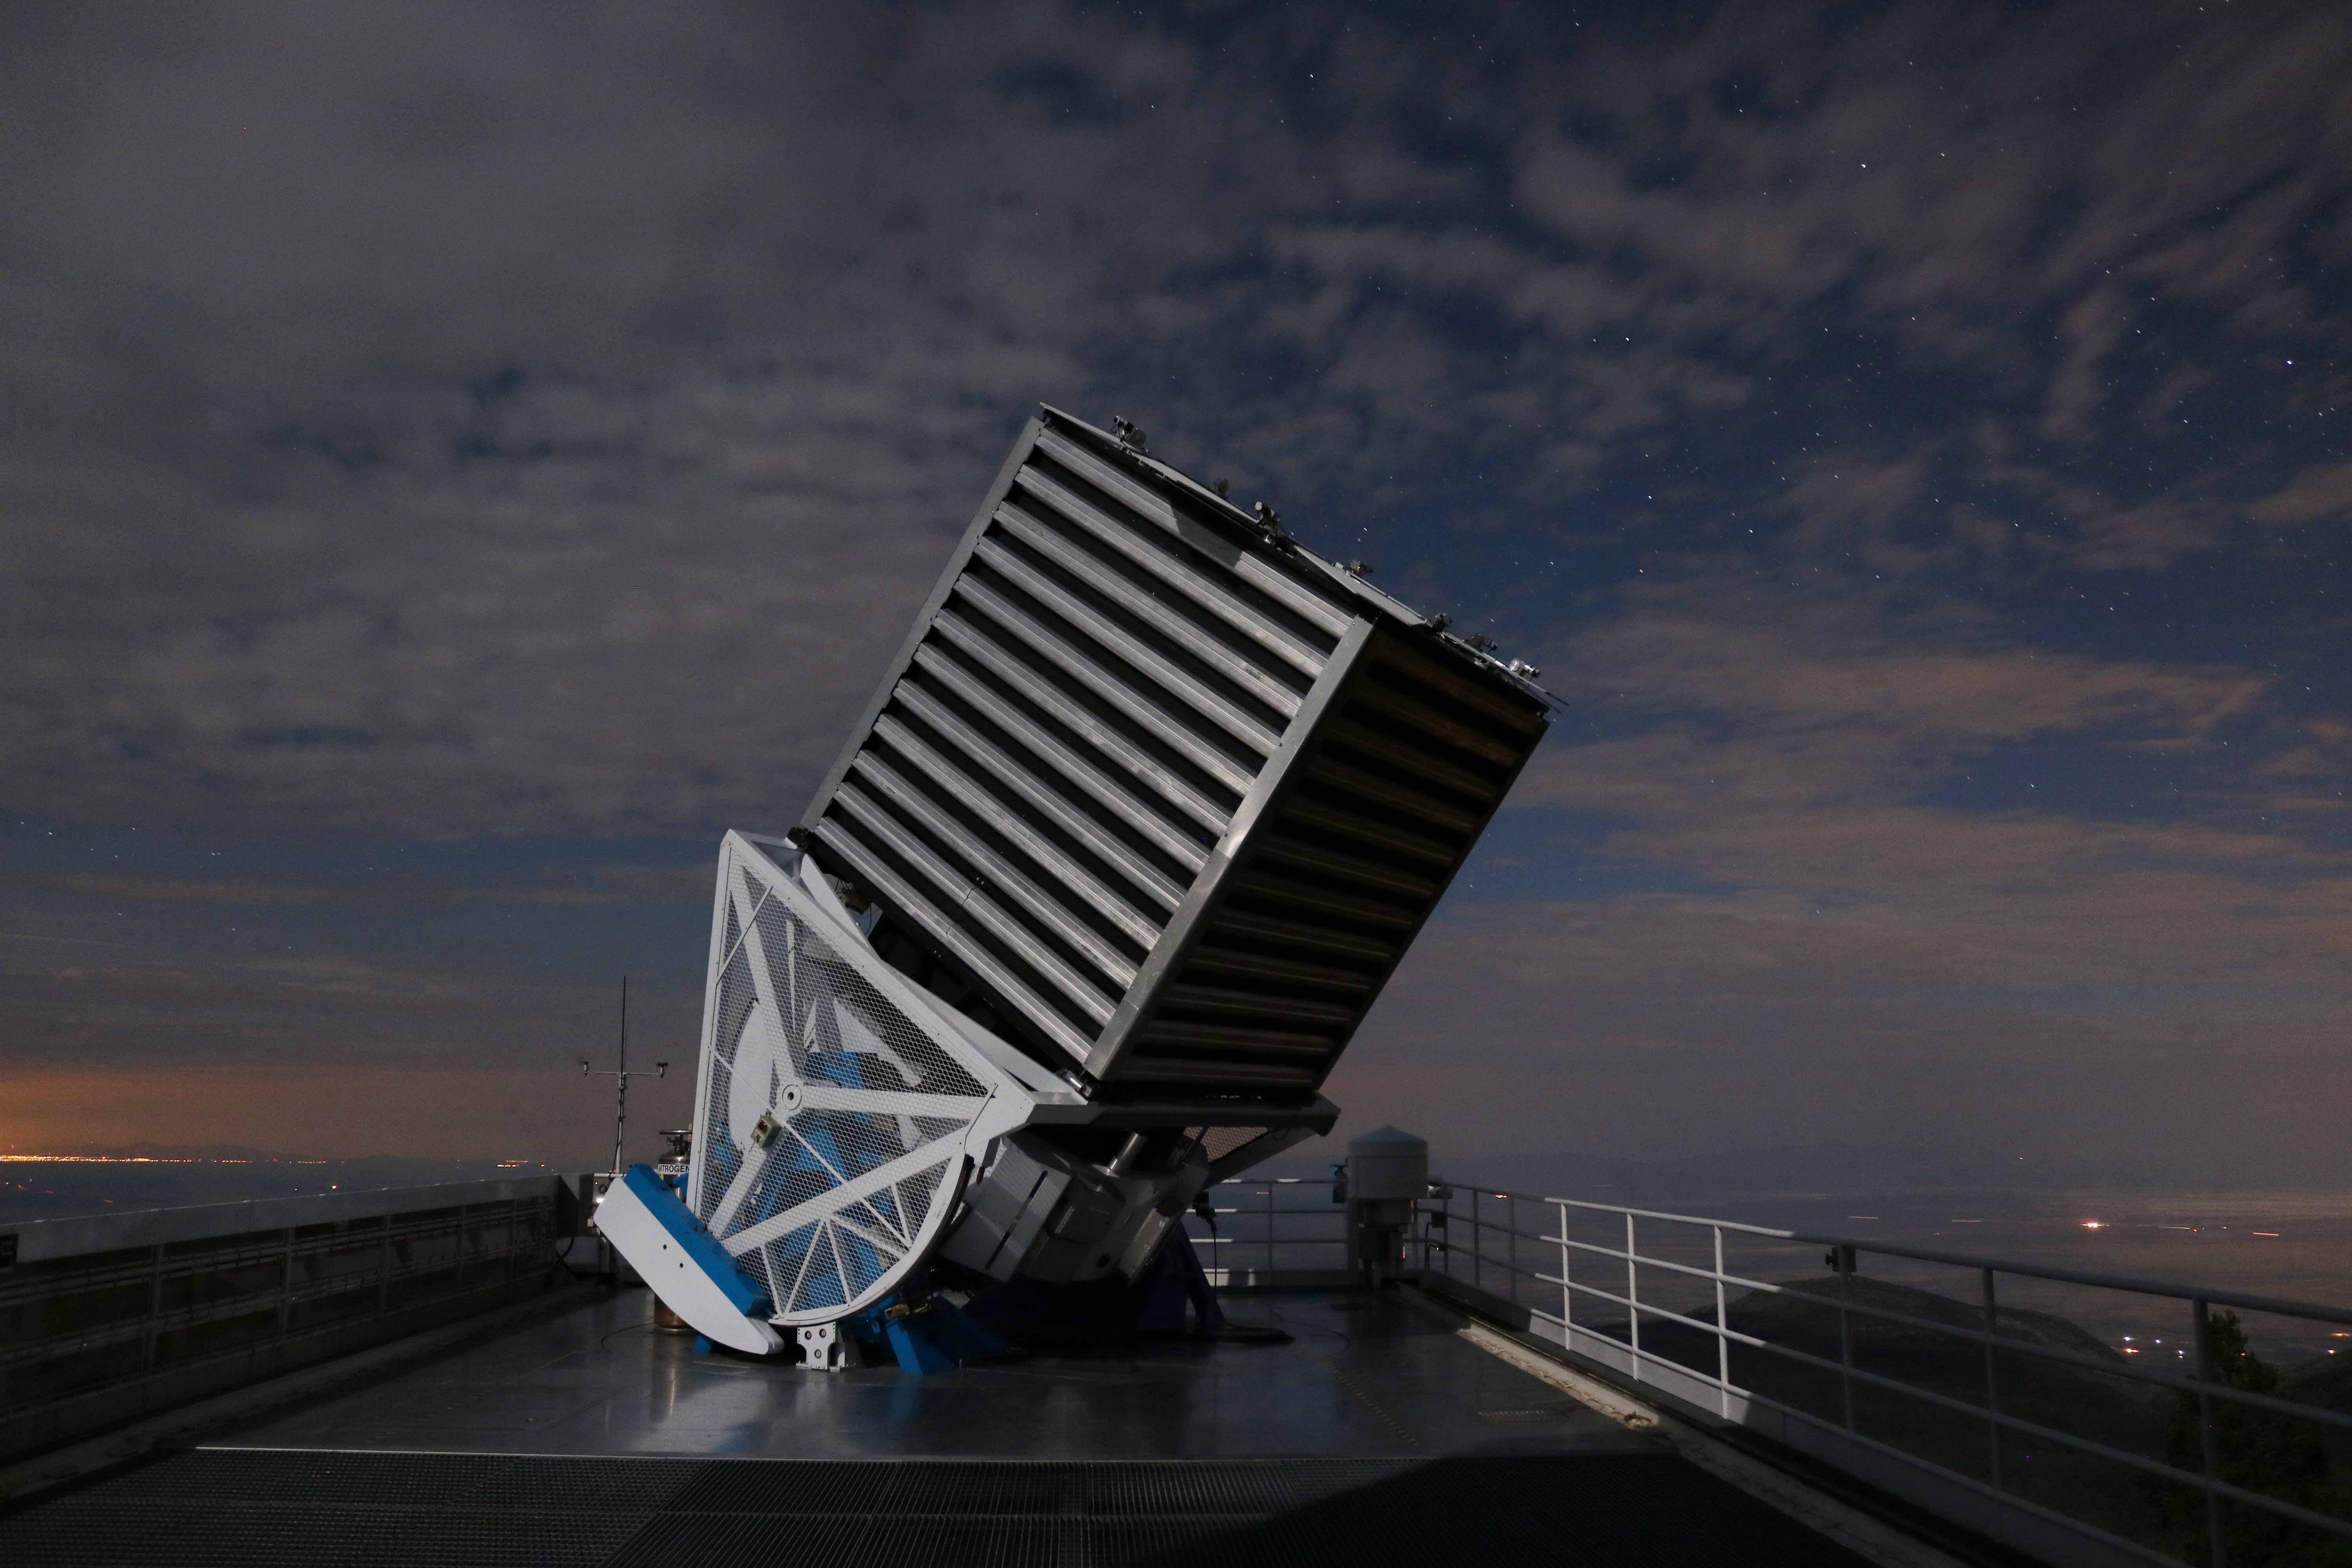
\includegraphics[width=\textwidth]{img/sdss_gaulme.jpg}
	\caption{The SDSS telescope at night (Image by Patrick Gaulme is licensed under CC BY 4.0)}
	\label{sdss_telescope}
\end{figure}

The SDSS Data Release 14 Quasar (DR14Q) catalog described in~\cite{paris2018}. % TODO add DR14Q acronym?
The DR14Q catalog contains 526\,356 quasars (contamination is estimated to be about 0.5\%).
% TODO what calibrated means?
% TODO define spectral resolution
SDSS provides calibrated spectra covering the wavelength range 3\,610--10\,140~\AA{} at a spectral resolution 1\,300 < \(R\) < 2\,500 for all the quasars.
The DR14Q catalog paper~\cite{paris2018} defines a quasar:

\begin{definition}
	A quasar is an object with a luminosity \(M_i[z = 2] < -20.5\)
	% TODO what is FWHM?
	and either displaying at least one emission line with FWHM > 500~km~s\(^{-1}\) or,
	if not, having interesting absorption features.
	\label{qso_definition}
\end{definition}

\subsection{Large Sky Area Multi-Object Fiber Spectroscopic Telescope}

Describe LAMOST, its spectra and catalog of QSOs.

The LAMOST is a special telescope with a primary mirror made of 37 hexagonal spherical mirros of total size 6.67~m times 6.05~m.
The large primary mirror makes the field of view of 5\(^{\circ}\).
The focal surface has 4000 fibers connected to 16 spectrographs with 32 CCD cameras.
Therefore, the telescope is capable of observing up to 4000 spectra simultaneously
in a wavelength coverage of 370--900~nm with spectral resolution \(R = 1000\) or \(R = 1500\) depending on gratings and camera positions.~\cite{cui2012}

One of the key scientific goals of LAMOST is the extragalactic spectroscopic survey of the large scale structure of the universe and the physics of galaxies.
The goal includes spectroscopic survey of nearly 10 millions galaxies and \textit{quasars}
that will contribute to the study of the accretion process of massive black holes in AGNs besides other things.~\cite{cui2012}

\section{Comparison of the Spectral Data}

Compare instruments, data and sky coverage.

Investigate the structure of data space in selected datasets (dimensionality reduction).
